\chapter{Evaluation}\label{chapter:evaluation}
The research topic of this thesis is how to best combine items (particularly regions) to improve travel recommendations. After much consideration and research, a genetic \gls{ea} was selected as the best algorithmic solution to the \gls{moop}. In this chapter, we describe the conducted experiments and their results. The experiments are presented in two parts. First, an online evaluation of the different algorithm variants is conducted. Then, we filter the results to eliminate some algorithm variants. The second part is the offline user survey. In the survey, participants are requested to rate different region combinations on a five-point Likert scale. In the following sections, the experimental setup as well as the online and offline studies are explained in depth.

\section{Experimental setup}
The experimental setup consists of combinations of elements of an approach that together form an algorithm variant. Figure \ref{fig:experiment_setup} how the various algorithmic approaches described in Section \ref{sec:impl} are combined to form six separate algorithm variants. Variant 1 is the baseline algorithm and is the closest to \gls{nsga}-III. Therefore, it can be described as an implementation of the unconstrained \gls{nsga}-III described in Part I of the \gls{nsga}-III paper \parencite{Deb2006ReferenceAlgorithms}.

\begin{figure}[h!]
    \centering
    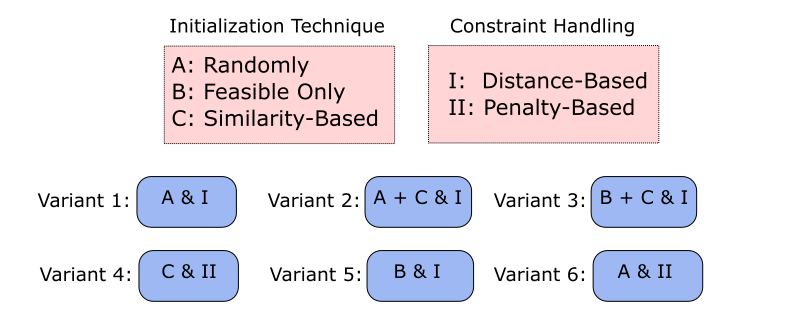
\includegraphics[width=.7\textwidth]{Experiment_Setup}
    \caption{Combination of algorithmic approaches to form algorithm variants}
    \label{fig:experiment_setup}
\end{figure}


Table \ref{tab:alg_parameters} summarizes the test setup parameters used for all variants. Each algorithm variant terminates at the 150$^{th}$ generation. This generation number for termination was selected because after several tests, it was discovered to be the limit to further improvement to the Pareto front. Moreover, unnecessary computational time that limits the usage of the \gls{rs} needed to be avoided. During the various test cases, the number of objectives $M$ was fixed at four. This number was chosen as it was considered sufficient to test the algorithms. In addition, increasing the number of objectives impacts the computational speed of the algorithm variants.

Each algorithm variant underwent 10 test runs for each sample input query. Three inputs (see \ref{tab:input_scenarios}) were carefully chosen to capture different travel preferences a user might have.

\begin{table}[htpb]
  \caption[Test Setup Parameters]{Constant test setup parameters for all algorithmic variants.}\label{tab:alg_parameters}
  \centering
  \begin{tabular}{l l}
    \toprule
       Parameter&Value  \\
    \midrule
      Maximum generation & 150  \\
      Number of divisions on every objective axis $p$& 12  \\
      Population Size $N$ (Variants 1, 2, 4, and 6) & 92   \\
       Population Size $N$ (Variant 3 and 5) & 40   \\
       Crossover operator & Two point \\
      Crossover probability $P_c$ & 0.3  \\
      Mutation operator & Flip bit \\
      Mutation probability $P_m$ & 1/length of input preferences \\
      Number of test runs per variant & 10\\
      Number of sample queries & 3\\
    \bottomrule
  \end{tabular}
\end{table}

\begin{table}[htpb]
\caption[Experiment Input Queries]{Input queries used for tests}\label{tab:input_scenarios}
  \centering
\begin{tabular}{ccccc}
\rowcolor[HTML]{005293} 
\cellcolor[HTML]{005293}{\color[HTML]{FFFFFF} }                        & \multicolumn{4}{c}{\cellcolor[HTML]{005293}{\color[HTML]{FFFFFF} Values}}                                                                                                                                                                                                                                                                                                                                                                                    \\ \cline{2-5} 
\rowcolor[HTML]{808080} 
\multirow{-2}{*}{\cellcolor[HTML]{005293}{\color[HTML]{FFFFFF} Input}} & \multicolumn{1}{c|}{\cellcolor[HTML]{808080}{\color[HTML]{FFFFFF} Preferences}}                                                               & \multicolumn{1}{c|}{\cellcolor[HTML]{808080}{\color[HTML]{FFFFFF} Budget}} & \multicolumn{1}{c|}{\cellcolor[HTML]{808080}{\color[HTML]{FFFFFF} \begin{tabular}[c]{@{}c@{}}Duration\\ in Weeks\end{tabular}}} & \multicolumn{1}{c|}{\cellcolor[HTML]{808080}{\color[HTML]{FFFFFF} Preferred Months}}          \\ \hline
\multicolumn{1}{|c|}{1}                                                & \multicolumn{1}{c|}{\begin{tabular}[c]{@{}c@{}}Beach,\\ Water sports,\\ Entertainment,\\ Culinary,\\ Safety from crime\end{tabular}}          & \multicolumn{1}{c|}{3,000}                                                  & \multicolumn{1}{c|}{3}                                                                                                          & \multicolumn{1}{c|}{July, August}                                                             \\ \hline
\multicolumn{1}{|c|}{2}                                                & \multicolumn{1}{c|}{\begin{tabular}[c]{@{}c@{}}Nature and Wildlife,\\ Hiking,\\ Culture\end{tabular}}                                         & \multicolumn{1}{c|}{6,000}                                                  & \multicolumn{1}{c|}{6}                                                                                                          & \multicolumn{1}{c|}{\begin{tabular}[c]{@{}c@{}}December, \\ January,\\ February\end{tabular}} \\ \hline
\multicolumn{1}{|c|}{3}                                                & \multicolumn{1}{c|}{\begin{tabular}[c]{@{}c@{}}Cities and Architecture,\\ Culture,\\ Culinary,\\ Shopping, \\ Safety from crime\end{tabular}} & \multicolumn{1}{c|}{4,000}                                                  & \multicolumn{1}{c|}{4}                                                                                                          & \multicolumn{1}{c|}{\begin{tabular}[c]{@{}c@{}}September,\\ October\end{tabular}}             \\ \hline
\end{tabular}
\end{table}

\section{Online Evaluation}
After several runs of the different algorithm variants, the goal of the online evaluation of the test results is to compare the effectiveness of each variant based on the following:
\begin{enumerate}
    \item How many regions is it able to combine as a single suggestion,
    \item The best total score from its list of suggested region combinations,
    \item Computational time required, and
    \item How diverse its suggestions are from other variants.
\end{enumerate}
 
\subsection{Algorithm Variants Comparison}
To compare the different algorithm variants, we present two perspectives of the results. First, we show the generational score of each variant. Then, we show the distribution of the obtained scores for each variant alongside the computational times.

In figure \ref{apx:fig:alg_comparison_generational}, the average feasible and infeasible scores at each generation are depicted for each variant with a 95\% confidence interval. The gray dotted line represents the constant average over all the feasible scores of all algorithm variants; it shows the minimum achievable score for each variant. Variants 1, 5, and 6 obtained average scores above the target line across generations. The distribution of scores for Variants 4 and 6 are very noisy. This can be explained by the heavy penalty values used by both variants. At first glance, we can infer that Variants 1, 5, and 6 are the best-performing variants. To make an informed decision, a second perspective on the results is presented.

\begin{figure}[h]
    \centering
    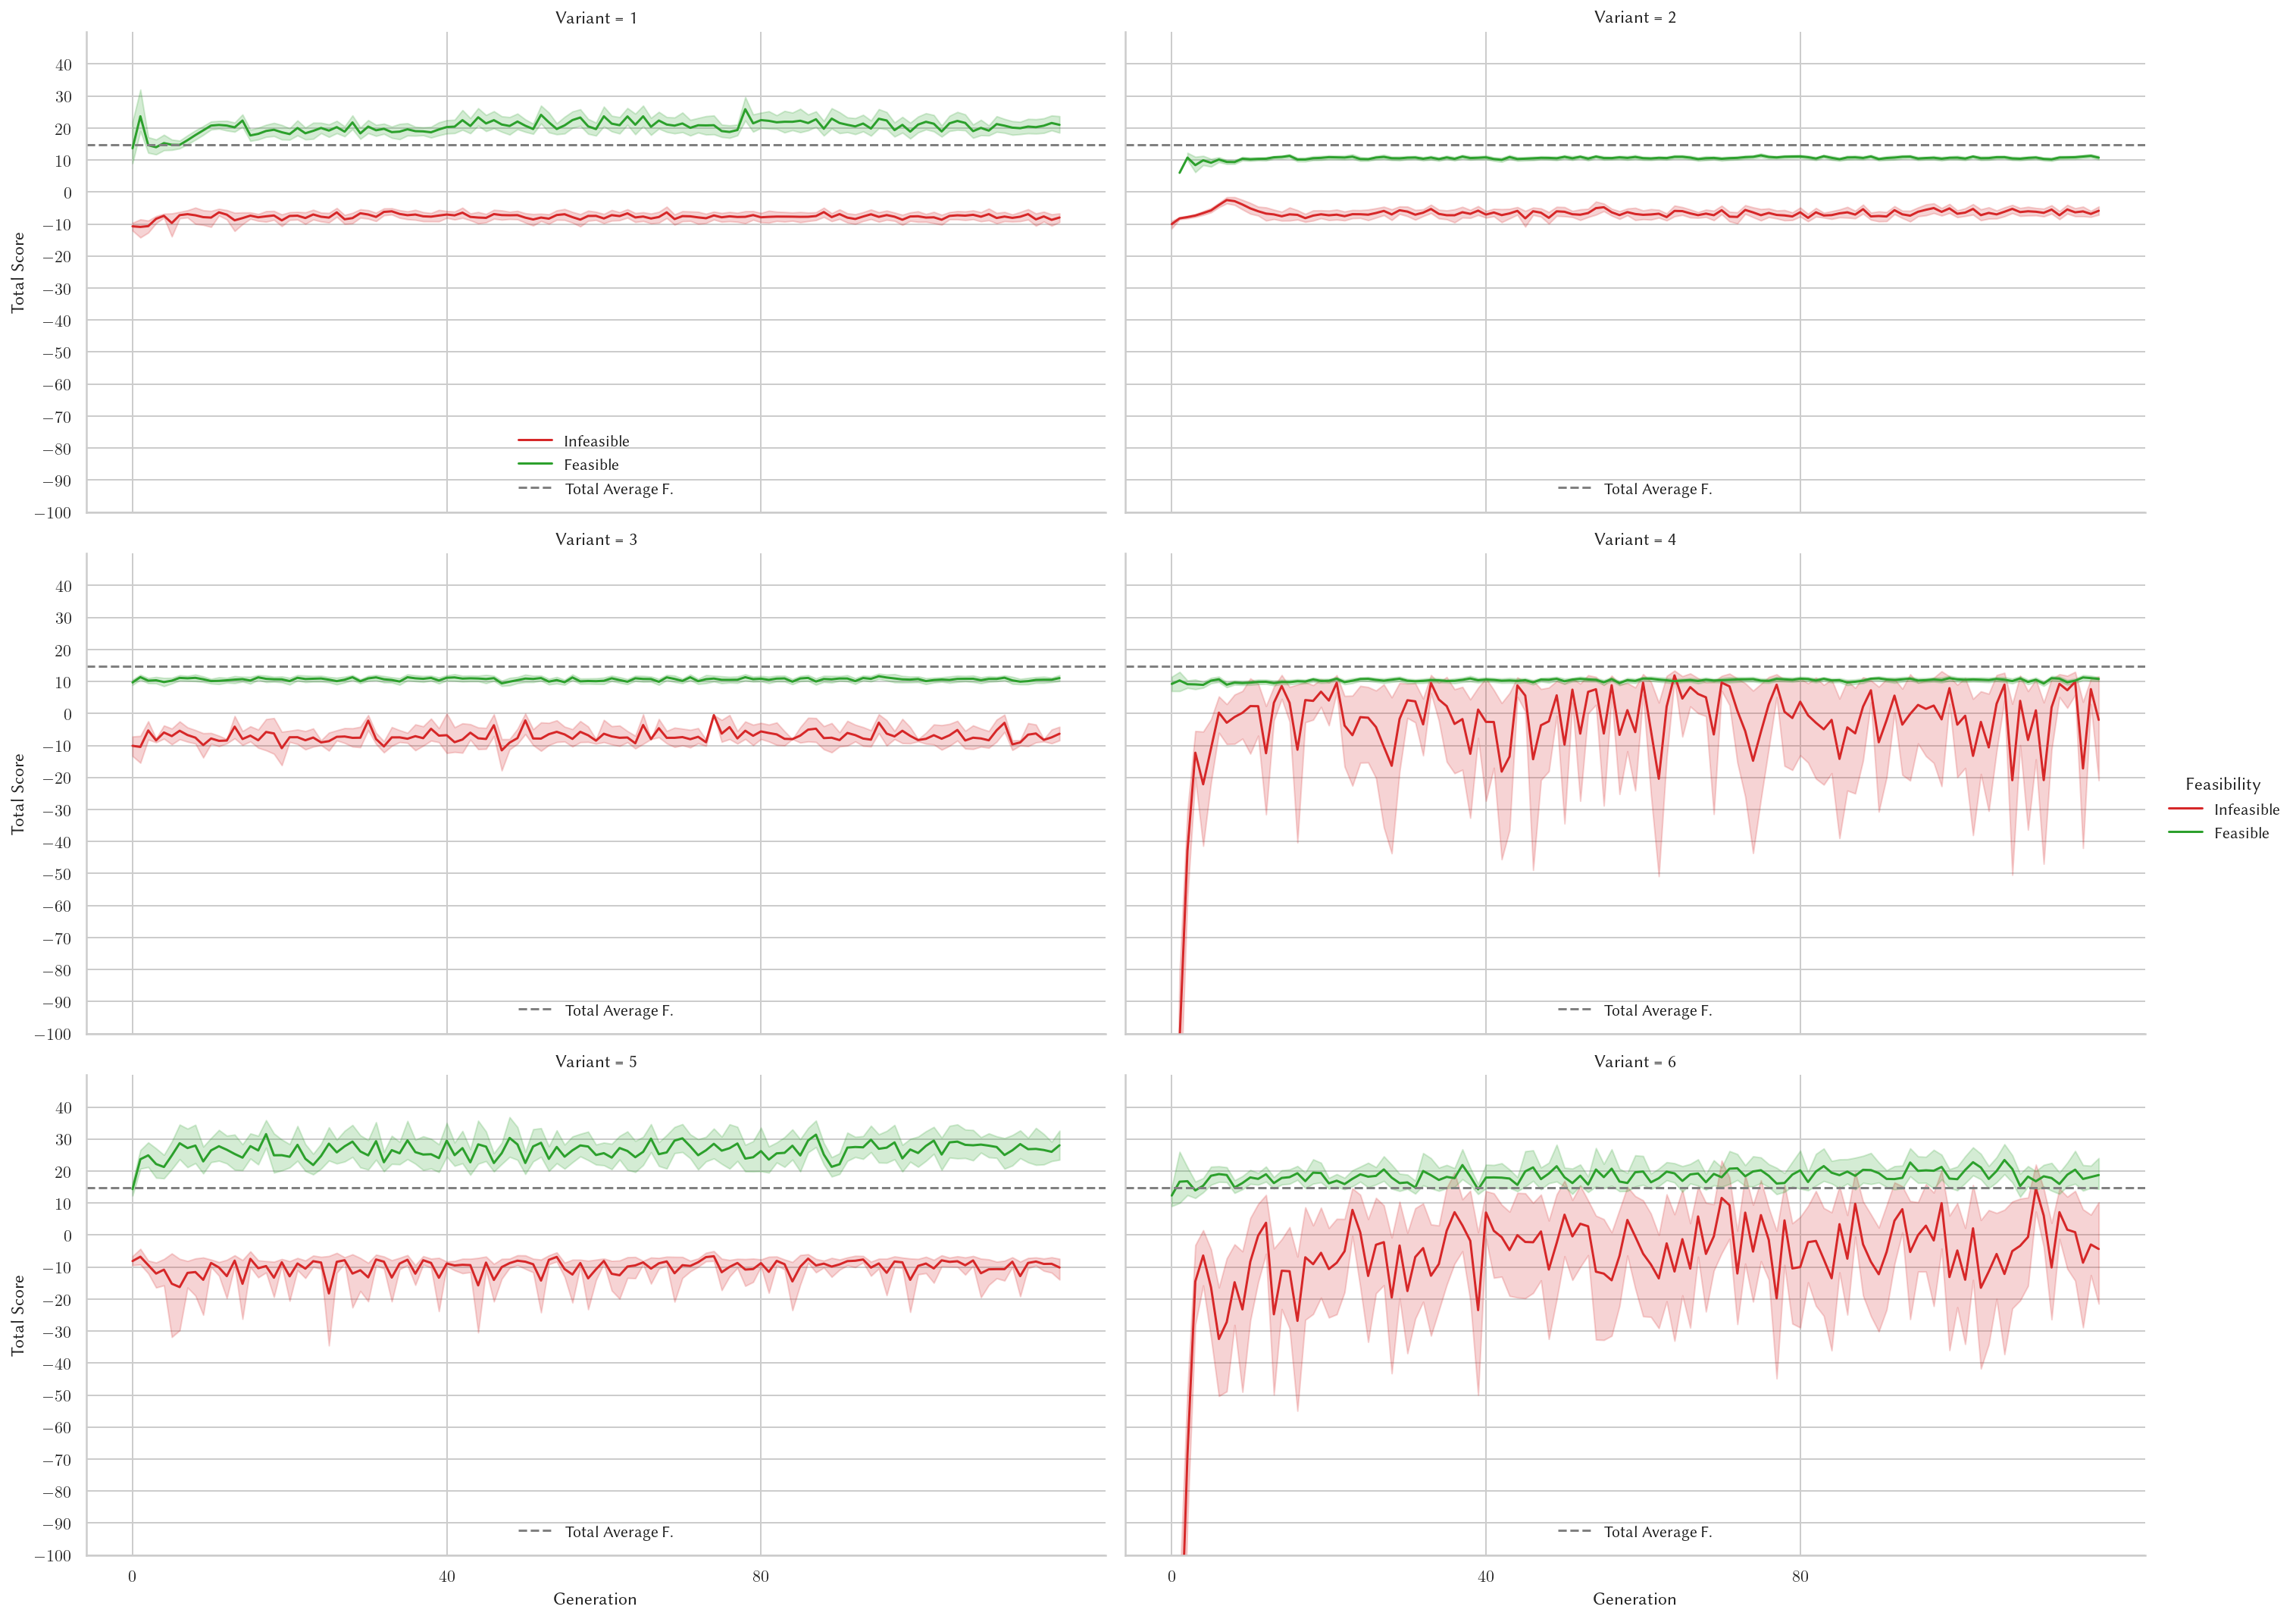
\includegraphics[width=\textwidth]{summarized_all_varaints}
    \caption[Average generational total score of all variants]{Average total score across generations. The gray dotted line represents a constant overall average score from all feasible combinations.}
    \label{apx:fig:alg_comparison_generational}
\end{figure}

Statistical data obtained through experiments showed that the scores generated by Variants
1, 4, and 5 outperform all other variants in terms of the average total score achieved. Figure \ref{fig:alg_comparison_online} shows the score (per combination) and the average time taken in seconds for each evaluated algorithm variant. On the $y$-axis, the color intensity corresponds to the average number of generated combinations per run. A gray dotted line on each variant indicates the average amount of computation time needed by the variant.

It is observed that Variant 3 requires the greatest amount of time (249.1s), while Variant 4 requires the least amount of time (71.4s). However, Variants 2, 3, and 4 are the worst-performing algorithms, having average scores of 10.3, 12.25, and 11.20, respectively. Variant 5, with an average score of 29.54, is statistically the best-performing algorithm. Variants 5 and 6 generated high numbers of region combinations. Variant 1 also generated high scores; however, its maximum obtained score is an outlier.

\begin{figure}[ht]
    \centering
    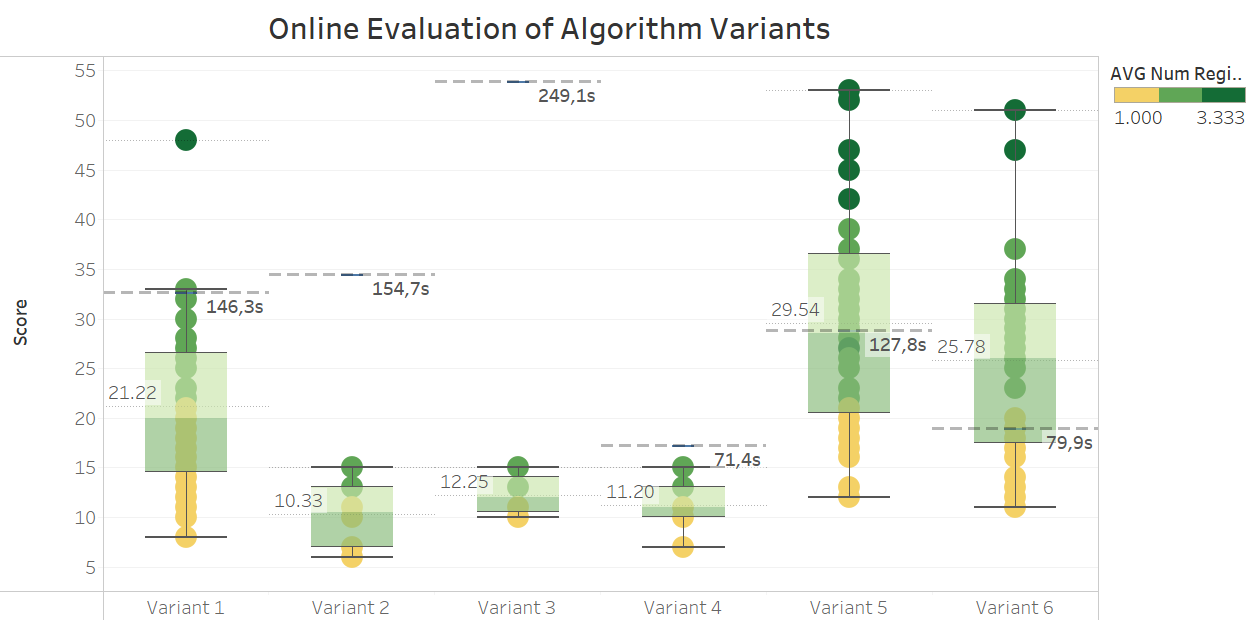
\includegraphics[width=\textwidth]{Online_Eval_Stats}
    \caption[Per Test Variant Online Experimentation Results]{Online Experimentation Results (For Values Table, see appendix \ref{tab:online_stats})}
    \label{fig:alg_comparison_online}
\end{figure}



\subsection{Results}
Informed by the two perspectives on the data from the experiments, we obtain a measure of the effectiveness of the variants as we discussed at the beginning of the online evaluation section. Variants 1, 5, and 6 rank the highest on all metrics and are able to suggest diverse region combinations. However, Variants 2, 3, and 4 suggest similar region combinations on most runs.

\begin{table}[h!]
\centering
\caption{Similarity in suggested region combination by variants}
\label{tab:sim_suggestions}

\begin{tabular}{|l|l|l|}
\hline
\textbf{Input} & \textbf{Variant} & \textbf{Suggested Regions} \\ \hline
1 & 2, 3, 4 & \begin{tabular}[c]{@{}l@{}}Central Africa, \\ Sahel East\end{tabular} \\ \hline
2 & 2, 3, 4 & \begin{tabular}[c]{@{}l@{}}Qatar and Bahrain,\\ Iraq and Kuwait\end{tabular} \\ \hline
3 & 2, 3, 4 & Greenland \\ \hline
\end{tabular}%

\end{table}

Table \ref{tab:sim_suggestions} shows the best region combinations suggested by the three variants. It is noteworthy that the best region combinations from the three low-ranking variants are exactly the same. A summary of the performance of the variants on each metric is presented in Table 5.4. We can conclude that Variants 1, 5, and 6 should be the selected variants for the offline evaluation. However, for diversity, a fourth variant was selected. The worst performing variant (Variant 2) was chosen as the extra variant for offline evaluation. Thus, results from Variants 1, 2, 5, and 6 are to be further evaluated in the user survey.



\begin{table}[h!]
  \caption[Algorithm Comparison]{Variants comparison of effectiveness Metrics}\label{tab:comparison_variants_sum}
  \centering
  \begin{tabular}{|c| c c c c| }
    \toprule
       &Computational time & \# Regions & Achievable Score & Non-Similarity\\ 
    \midrule
       Variant 1& &\checkmark  &\checkmark & \checkmark \\ \hline
      Variant 2&  &  & & \\ \hline
      Variant 3& & & &  \\ \hline
      Variant 4& \checkmark &  & & \\ \hline
      Variant 5& \checkmark &\checkmark  &\checkmark & \checkmark \\ \hline
      Variant 6& \checkmark &\checkmark  &\checkmark & \checkmark \\ 
    \bottomrule
  \end{tabular}
\end{table}



\section{Offline Evaluation}
The offline evaluation was designed with the aim of evaluating the performance of the 4 designed variants of the genetic evolutionary algorithm. We conducted a study comprising participants of varying travelling knowledge. Respondents were giving the opportunity to evaluate for their preferred travel styles.
\subsection{Procedure of the Survey}
The user survey was composed of suggested region combinations and minimum stay durations obtained from algorithm Variants 1 (baseline), 4, 5, and 6. Region combinations having the highest score from each variant were used for the three sample input queries (scenarios shown in Table \ref{tab:input_scenarios}) presented to the respondents. A typical region combination was shown to the participants as presented in Figure \ref{fig:suggestion}. 

\begin{figure}[h]
    \centering
    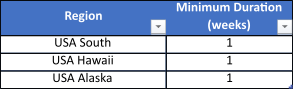
\includegraphics[width=.5\textwidth]{Alg5_input1}
    \caption[Suggested region combinations and stay durations from Variant 5 as presented to participants]{Suggested region combinations and stay durations from Variant 5 as presented to participants (all presented combinations can be seen in appendix figures \ref{fig:input1_suggestions}, \ref{fig:input2_suggestions}, \& \ref{fig:input3_suggestions})}
    \label{fig:suggestion}
\end{figure}

First, the participants were asked general background information about their travel knowledge and styles. Specifically, they questioned regarding the following:
\begin{enumerate}
    \item How often they travel;
    \item How good they are at planning travels,
    \item Their preferred travel activities from a list of activities, and
    \item Their level of trust. 
\end{enumerate}
This allowed us to match the travelers to the travel scenarios and also to categorize them as advanced, basic, or average travelers.

In total, 12 suggested region combinations were presented to the participants, and they were asked to rate each suggestion on a five-point Likert scale ranging from 1 to 5 (strongly disagree to strongly agree). Point 0 was reserved for participants who did not relate to the travel scenario. The participants rated each recommendation based on the following:
\begin{enumerate}
    \item Accuracy of the suggestion,
    \item Overall satisfaction with the suggestion,
    \item How well the regions fit together (i.e, cohesiveness), and
    \item Diversity of the recommendations.
\end{enumerate}

Table \ref{tab:survey_questions} in the appendix describes the specific wording of the survey questions and the response types for each category.

\subsection{Results}
A total of 104 participants with varying travel knowledge took part in the survey. Each participant could relate to at least two of the input scenarios (i.e., minimum of 204 responses per variant). Hence, we evaluated each algorithm variant on at least two travel types. Figure \ref{fig:survey_overview} compares the algorithm variants based on the responses obtained on a diverging bar chart.

\begin{figure}[ht]
    \centering
    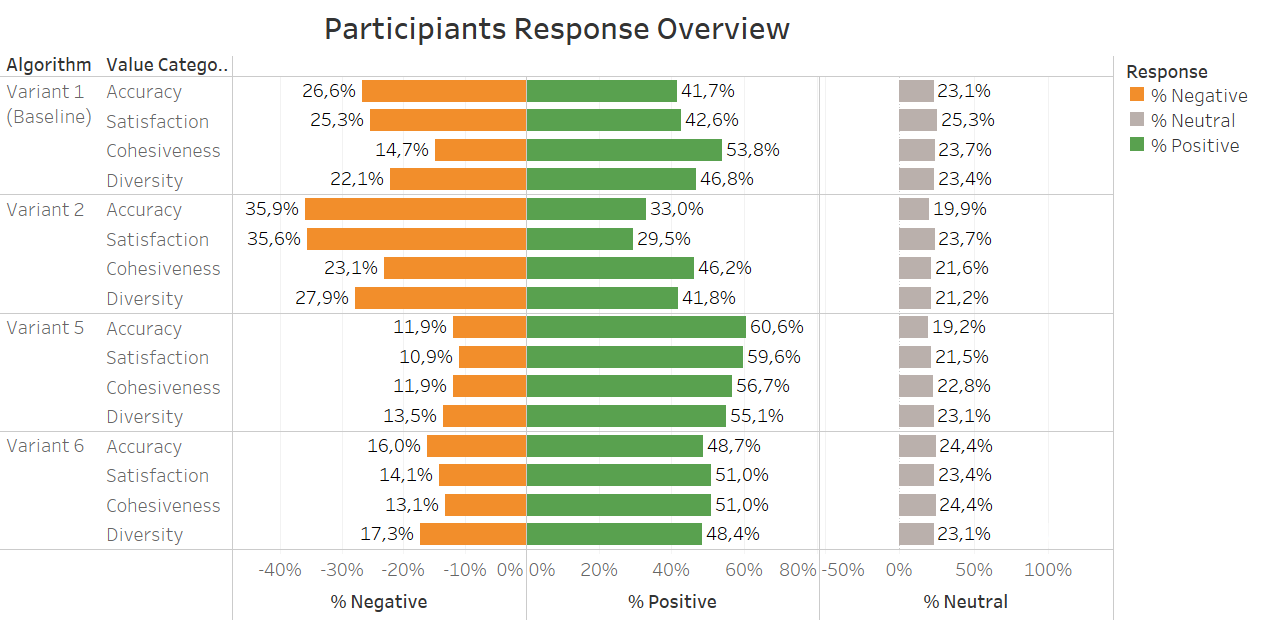
\includegraphics[width=\textwidth]{Survey_Overview_Per_Variant}
    \caption[Comparison of the algorithm variants based on responses obtained per variant on each question category]{Comparison of the algorithm variants based on responses obtained per variant on each question category. Please note that negative signs on the axis only represent the direction of the diverging chart.}
    \label{fig:survey_overview}
\end{figure}

Each row represents the results for an algorithm variant, and this is further grouped based on the question categories. On the $x$-axis, the responses are grouped into percentage negative, percentage positive, and percentage neutral. For each question category, the percentage negative represents the percentage of the total responses regarding a particular variant with ratings less than 3 ($(0, 2]$). Percentage positive represents ratings from 4 to 5 ($[4,5]$) on a question category. Participants who rated a suggestion with the value of 3 were considered neutral to ensure that we could accurately rate responses as positive or negative.


From the diverging chart, it can be observed that Variant 5 was the best-performing variant relative to baseline. More than half of the respondents rated it highly in all question categories. It ranked highest in accuracy, satisfaction, cohesiveness, and diversity. An improvement in accuracy, 39.8\% improvement in satisfaction, 5.5\% in cohesiveness, and 17.8\% in diversity was achieved relative to the baseline for this variant. Compared to other variants in each category, no variant performed better than Variant 5.

Variant 2 performed worse than baseline on all metrics. It ranked last in overall satisfaction, followed by accuracy, diversity, and cohesiveness. It showed a 20.8\% decrease in accuracy, a 30.8\% decrease in satisfaction, a 14.3\% decrease in cohesiveness, and a 10.6\% decrease in diversity relative to the baseline.

Variant 6 was the second-best performing variant; 48.7\% of the respondents found it accurate, and 51\% were satisfied with its results. However, compared to baseline, it performed worse in terms of cohesiveness of region combinations.

\begin{figure}[htpb]
    \centering
    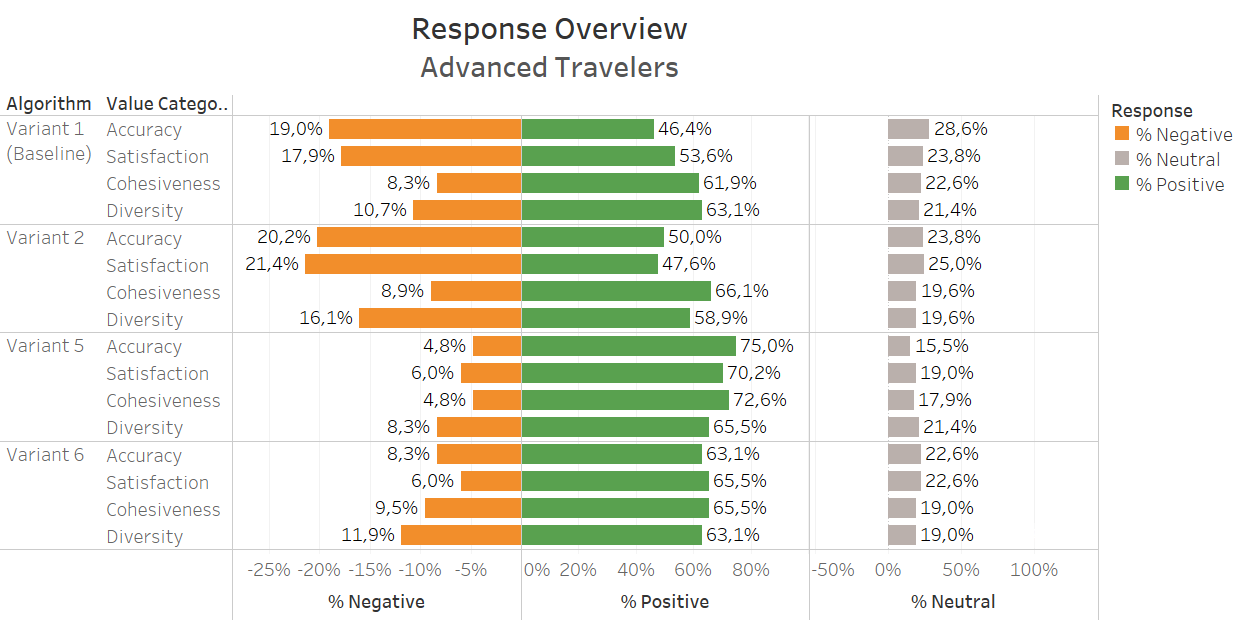
\includegraphics[width=\textwidth]{Survey_Advanced_Travelers_Results}
    \caption{Response overview filtered by travel knowledge of participants – Advanced Knowledge Travelers Only}
    \label{fig:survey_advanced_travelers}
\end{figure}

A Kruskal-Wallis \parencite{Vargha1998TheHomogeneity} test was computed to determine whether there is a statistically significant difference between the median ratings of the algorithm variants concerning the responses gotten from the survey. For better test accuracy, we did not take neutral responses into account. The test showed a significant difference (p $\leq$ 0.001) between the algorithm variants with regard to the ratings by the respondents. As a consequence of the statistically significant results from the Kruskal-Wallis test, a Dunn's test was conducted to determine the significance level between the variant pairs. Table \ref{tab:dunntest} reveals the results of the test. There is a significant difference between all algorithm variants. The pairs of Variant 1 and 6 and the pairs of Variant 5 and 6 are less different from each other. However, using a significance level of 0.05, all variant pairs are statistically significantly different from one another,

\begin{table}[h]
\centering
\caption[Dunn-Bonferroni-Tests for pairwise comparison of the level of significance between the algorithm variants]{ Dunn-Bonferroni-Tests for pairwise comparison of the level of significance between the algorithm variants. It tells us which variants are statistically significantly different. Adj. p: Values adjusted with Bonferroni correction}
\label{tab:dunntest}
\resizebox{\textwidth}{!}{%
\begin{tabular}{|l|l|l|l|l|l|}
\hline
\multicolumn{1}{|c|}{} & \textbf{Test Statistic} & \textbf{Std. Error} & \textbf{Std. Test Statistic} & \textbf{p} & \textbf{Adj. p} \\ \hline
Variant 1 - Variant 2 & 292.41  & 44.88 & 6.52   & \textless{}.001 & \textless{}.001 \\ \hline
Variant 1 - Variant 5 & -248.62 & 42.47 & -5.85  & \textless{}.001 & \textless{}.001 \\ \hline
Variant 1 - Variant 6 & -138.4  & 43.29 & -3.2   & .001            & .006            \\ \hline
Variant 2 - Variant 5 & -541.03 & 44.65 & -12.12 & \textless{}.001 & \textless{}.001 \\ \hline
Variant 2 - Variant 6 & -430.81 & 45.43 & -9.48  & \textless{}.001 & \textless{}.001 \\ \hline
Variant 5 - Variant 6 & 110.22  & 43.05 & 2.56   & .01             & .042            \\ \hline
\end{tabular}%
}
\end{table}

We created travel knowledge categories for the participants according to their travel planning ability and travel experience. Participants with travel experience and planning abilities above three were categorized as advanced travelers. Participants who rated their travel experience and planning ability below two were classified as basic travelers. All other travel experiences and travel planning ability rating combinations were categorized as having average travel knowledge.

An interesting observation made when filtering the responses for advanced travelers only (\ref{fig:survey_advanced_travelers}) was that compared to baseline, travelers with more than average travel knowledge were more satisfied with the cohesiveness and accuracy of the region suggestions from Variant 2. Furthermore, based on the positive responses of advanced travelers, Variant 6 performed at least as good as the baseline in terms of diversity and better than the baseline in terms of accuracy, satisfaction, and cohesiveness.

This insight from the responses of advanced travelers is crucial because they tend to have more travel domain knowledge.  A second Kruskal-Wallis test was conducted to test if this observed difference in the responses by travelers with advanced knowledge and other traveler is statistically significant. The test revealed that there is a significant difference (p $\leq$ 0.001) between the advanced, average, and basic travelers with respect to their response values. Figure \ref{fig:stats_sig_all_knowledge} illustrates a side-by-side comparison of the ratings of all algorithm variants by advanced, average, and basic travelers. It is evident that advanced travelers are more generous with their evaluations than all other travel knowledge categories.

\begin{figure}[ht]
    \centering
    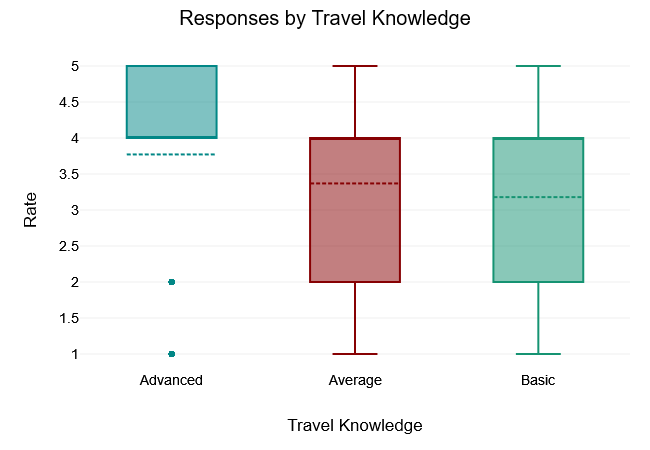
\includegraphics[width=.7\textwidth]{Response_by_knowledge.png}
    \caption{Side-by-Side comparison of ratings from advanced, average, and basic travelers}
    \label{fig:stats_sig_all_knowledge}
\end{figure}

\section{Discussion}
The results obtained from the offline evaluation are in line with the results obtained through the online evaluation of the variants. As demonstrated above, Variants 5 and 6 were the best-performing algorithm variants, while Variant 2 was the worst-performing variant. Therefore, the overall performance of the algorithm variants is directly dependent on the performance of the variants in the online evaluation.


Variant 6 was unable to improve baseline in terms of cohesiveness. However, advanced travelers rated Variant 6's suggestions as more cohesive than baseline. From the results of the second Kruskal-Wallis test, there is a statistically significant difference between advanced
travelers and all other travel knowledge categories. For participants to provide more precise evaluations of the cohesiveness of the regions, they must have good travel domain knowledge. Advanced travelers tend to have a better understanding of how the regions fit together. Thus, we cannot totally rule out Variant 6 because of its lower score in the category of cohesiveness. Moreover, Variant 6 took the least computational time of all the algorithm variants ($\phi$ 79.9s), and a fast computational time is vital to ensure the usefulness of a \gls{rs}. Hence, we can conclude that overall, Variant 5, Variant 6, and Variant 1 rank the highest.


\section{Implications}
The results from this evaluation reveal the high potential of initializing the start population with feasible individuals only. A large portion of the computational time used by the feasibility-based method is spent searching for feasible individuals. The tests performed in this work used a random search method. A hypothesis is that an efficient search heuristic would significantly improve the time performance of the feasibility-based initialization method. In Section \ref{sec:alg_approaches} various search heuristics such as the iterative local search, \gls{ts}, and others were explained. The computational time for the evolutionary process with the feasibility-based approach is shorter because a smaller population size is used. Therefore, improving the start population search process will significantly improve the computational speed of the algorithm.

Additionally, penalty-based constraint handling has proven effective, as shown in the evaluation of algorithm Variant 6. A new variant that uses a combination of a feasibility-based initialization and penalty-based constraint-handling of future offspring could provide effective results.

The computational speed of the other algorithm variants can still be improved through further tests. A high population number and a high maximum generation have a negative influence on the computational time of the evolutionary algorithm in general. Additional experiments must be conducted to test the trade-off limit between population number and the maximum generation that provide acceptable item combinations.




